\documentclass[aspectratio=169, 14pt]{beamer}
\usepackage[utf8]{inputenc}
\usepackage[english]{babel}
\usepackage{tipa}
\newcommand{\RNum}[1]{\uppercase\expandafter{\romannumeral #1\relax}}
\usepackage{graphicx}
\usepackage{transparent}
\usepackage[ruled, lined, linesnumbered, commentsnumbered]{algorithm2e}
\usepackage{pgfplots}
\newcommand\mycommfont[1]{\small\ttfamily\textcolor{blue}{#1}}
\SetCommentSty{mycommfont}
\renewcommand{\thealgocf}{}
\usepackage{setspace}
\usepackage{tikz}
\usetikzlibrary{matrix,backgrounds}
\usetikzlibrary{arrows}
\usetikzlibrary {arrows.meta}
\usetikzlibrary{calc,shadows.blur,fit,positioning}
\usetikzlibrary{shapes.multipart,chains}
\usepackage{minted}
\usepackage{fontawesome5}
\usepackage{booktabs}
\usepackage{caption}
\usepackage{bookmark}
\usepackage{tabularray}
\usepackage{hyperref}
\hypersetup{
	colorlinks=true,
	linkcolor=blue,
	filecolor=magenta,
	urlcolor=cyan,
}
\urlstyle{same}
\usetheme{metropolis}
\metroset{block=fill}
\usecolortheme{default}
\definecolor{darkmidnightblue}{rgb}{0.0, 0.2, 0.4}
\definecolor{LightGray}{gray}{0.9}


%------------------------------------------------------------
%This block of code defines the information to appear in the
%Title page
\title[Data Structures] %optional
{Data Structures}

\subtitle{Graph}

\author[CHEN Zhongpu] % (optional)
{CHEN Zhongpu}

\institute[] % (optional)
{
	School of Computing and Artificial Intelligence \\
	\href{mailto:zpchen@swufe.edu.cn}{zpchen@swufe.edu.cn}
}

\date[] % (optional)
{SWUFE, Fall \the\year{}}

%End of title page configuration block
%------------------------------------------------------------


%------------------------------------------------------------
%The next block of commands puts the table of contents at the 
%beginning of each section and highlights the current section:

% \AtBeginSection[]
% {
%   \begin{frame}
%     \frametitle{Table of Contents}
%     \tableofcontents[currentsection]
%   \end{frame}
% }
%------------------------------------------------------------


\begin{document}

%The next statement creates the title page.
\frame{\titlepage}

%---------------------------------------------------------
%This block of code is for the table of contents after
%the title page
% \begin{frame}
% \frametitle{Table of Contents}
% \tableofcontents
% \end{frame}
%--------------------------------------------------------

{
	% \usebackgroundtemplate{\transparent{0.3}{\begin{picture}
	%     \includegraphics[height=0.7\paperheight]{cover}
	% \end{picture}    
	% }}
	\usebackgroundtemplate{
		\tikz[overlay,remember picture]
		\node[opacity=0.3, at=(current page.south east),anchor=south east, yshift=2cm,xshift=4cm] {
			\includegraphics[height=0.6\paperheight]{cover}};
	}
	\begin{frame}
		\section{\textcolor{darkmidnightblue}{Graph}}
	\end{frame}

}

\begin{frame}[fragile]
	Trees are used to represent \alert{hierarchical} data. What if we want to represent non-hierarchical data?
	\begin{columns}
		\column{0.4\textwidth}
		\begin{enumerate}
			\item Maps
			\item Social networks
			\item Web pages
		\end{enumerate}
		\column{.6\textwidth}
		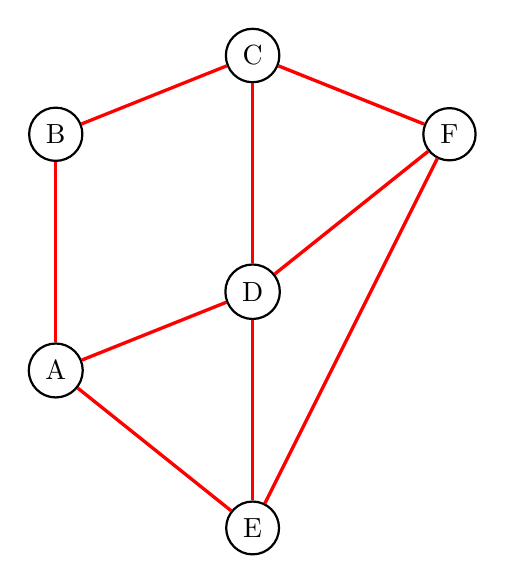
\begin{tikzpicture}
			\begin{scope}[every node/.style={circle,thick,draw}]
				\node (A) at (0,0) {A};
				\node (B) at (0,3) {B};
				\node (C) at (2.5,4) {C};
				\node (D) at (2.5,1) {D};
				\node (E) at (2.5,-2) {E};
				\node (F) at (5,3) {F} ;
			\end{scope}

			\begin{scope}[>={Stealth[black]},
				every node/.style={fill=white,circle},
				every edge/.style={draw=red,very thick}]
				\path  (A) edge  (B);
				\path  (B) edge  (C);
				\path  (A) edge  (D);
				\path  (D) edge  (C);
				\path  (A) edge  (E);
				\path  (D) edge  (E);
				\path  (D) edge  (F);
				\path  (C) edge  (F);
				\path (E) edge (F);
			\end{scope}
		\end{tikzpicture}
	\end{columns}

\end{frame}

\begin{frame}{1. Undirected Graph}

	\begin{exampleblock}{Graph}
		A graph is a set of \alert{vertices} and a collection of \alert{edges} that each connect a pair of vertices.
	\end{exampleblock}

	By convention, we use the names $0$ through $V-1$ for the vertices in a $V$-vertex graph.

	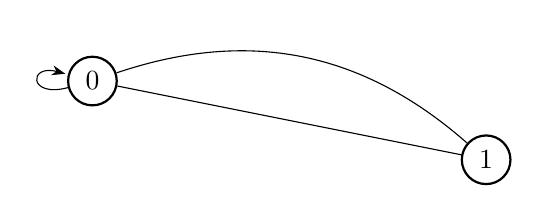
\begin{tikzpicture}
		\begin{scope}[every node/.style={circle,thick,draw}]
			\node (A) at (0,0) {0};
			\node (B) at (5,-1) {1};
		\end{scope}

		\begin{scope}[>={Stealth[black]}]
			\draw (A) -- (B);
			\path (A) edge [loop left] (A);
			\draw (A) edge [bend left] (B);
		\end{scope}
	\end{tikzpicture}
\end{frame}

\begin{frame}{1.1 Glossary}
	When there is an edge connecting two vertices, we say that the vertices are \alert{adjacent} to one another and that the edge is \alert{incident} to both vertices. The \alert{degree} of a vertex is the number of edges incident to it.

	\begin{enumerate}
		\item \alert{path}
		\item \alert{cycle}
		\item \alert{simple path}
		\item \alert{length}
	\end{enumerate}
\end{frame}

\begin{frame}[fragile]
	Is this a graph?

	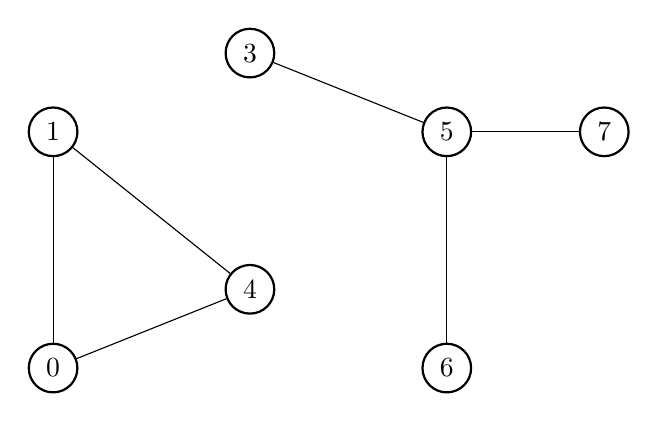
\begin{tikzpicture}
		\begin{scope}[every node/.style={circle,thick,draw}]
			\node (A) at (0,0) {0};
			\node (B) at (0,3) {1};
			\node (C) at (2.5,4) {3};
			\node (D) at (2.5,1) {4};
			\node (E) at (5,3) {5} ;
			\node (F) at (5,0) {6} ;
			\node (G) at (7,3) {7} ;
		\end{scope}

		\begin{scope}[>={Stealth[black]},]
			\draw (A) -- (B);
			\draw (B) -- (D);
			\draw (A) -- (D);

			\draw (C) -- (E);
			\draw (E) -- (G);
			\draw (E) -- (F);
		\end{scope}
	\end{tikzpicture}

	Try to understand the definition of a \alert{connected} graph, and \alert{connected component} by searching from the Internet.
\end{frame}

\begin{frame}{Quiz: graph and tree}
	Which of the following statements are true?

	\begin{enumerate}
		\item A tree is a graph.
		\item If a graph with $V$ vertices has $V-1$ edges, then it is a tree.
		\item If a graph with $V$ vertices has $V-1$ edges and is connected, then it is a tree.
		\item If a graph with $V$ vertices has $V-1$ edges and is acyclic, then it is a tree.
	\end{enumerate}
\end{frame}

\begin{frame}{1.2 Undirected graph ADT}
	\begin{table}
		\begin{tabular}{|l|l|}
			\hline
			method                & meaning                                        \\
			\hline
			\alert{Graph(V)}      & \textit{create a V-vertex graph with no edges} \\
			\alert{V()}           & \textit{number of vertices}                    \\
			\alert{E()}           & \textit{number of edges}                       \\
			\alert{addEdge(v, w)} & \textit{add an edge v-w}                       \\
			\alert{adj(v)}        & \textit{vertices adjacent to v}                \\
			\hline
		\end{tabular}
		\caption{Undirected graph API}
	\end{table}
\end{frame}

\begin{frame}{Exercise}
	Please design the following methods for the undirected graph ADT.

	\begin{itemize}
		\item \alert{degree(v)}: the degree of vertex $v$.
		\item \alert{numberOfSelfLoops()}: the number of self loops.
	\end{itemize}
\end{frame}

\begin{frame}[fragile]
	\frametitle{1.3 Representation alternatives}
	Basically, we have two ways to represent a graph.
	\begin{enumerate}
		\item \alert{Adjacency-matrix representation}: use a $V \times V$ matrix to represent a graph with $V$ vertices.
		\item \alert{Adjacency-lists representation}: use array of lists of the vertices adjacent to each vertex to represent a graph with $V$ vertices.
	\end{enumerate}

	
\begin{tikzpicture}
		\node[fill=yellow,blur shadow={shadow xshift=-0.5ex},
			text width=26em,anchor=south west,rounded corners]
		{Consider the trade-off between \alert{space} and \alert{time}.};
	\end{tikzpicture}
\end{frame}

\begin{frame}{Performance}
	\begin{table}
		\begin{tblr}{colspec={cllll},hlines}
			{underyling                                                      \\ data structure} & space & add edge & check \newline adjacency & iterate \newline over adjs \\
			\alert{adjacency matrix} & $V^2$ & 1 & 1           & $V$         \\
			\alert{adjacency lists}  & $E+V$ & 1 & $degree(v)$ & $degree(v)$ \\
		\end{tblr}
		\caption{Order-of-growth Performance of graph representations}
	\end{table}
\end{frame}

\begin{frame}[fragile]
	\frametitle{Exercise (1)}
	\begin{columns}
		\column{0.4\textwidth}

		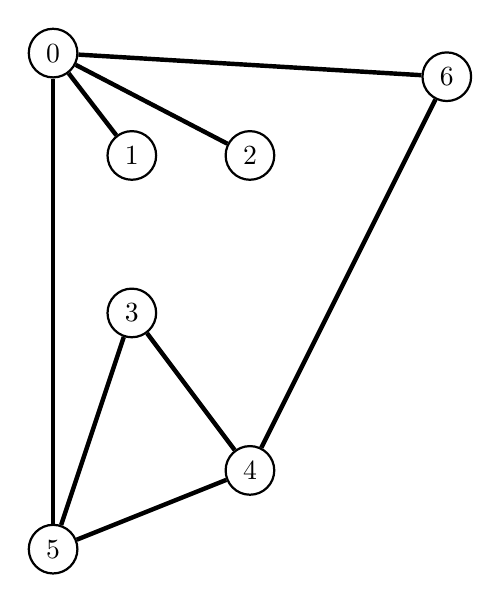
\begin{tikzpicture}
			\begin{scope}[every node/.style={circle,thick,draw}]
				\node (A) at (0,3.3) {0};
				\node (B) at (1,2) {1};
				\node (C) at (2.5,2) {2};
				\node (D) at (1,0) {3};
				\node (E) at (2.5,-2) {4};
				\node (F) at (0,-3) {5} ;
				\node (G) at (5, 3) {6} ;
			\end{scope}

			\begin{scope}[>={Stealth[black]},
				every node/.style={fill=white,circle},
				every edge/.style={draw, ultra thick}]
				\path  (A) edge  (B);
				\path  (A) edge  (C);
				\path  (E) edge  (D);
				\path  (A) edge  (F);
				\path  (F) edge  (E);
				\path  (F) edge  (D);
				\path  (A) edge  (G);
				\path  (G) edge  (E);
			\end{scope}
		\end{tikzpicture}

		\column{0.6\textwidth}
		Please draw the adjacency-lists representation of this graph.
	\end{columns}
\end{frame}


\begin{frame}[fragile]
	\frametitle{Exercise (2)}
	Given an undirected graph, which of the following statements are true?

	\begin{enumerate}
		\item The sum of degrees of all vertices is even.
		\item The number of edges is greater than the number of vertices minus 1.
		\item There is at least one vertex whose degree is 1.
	\end{enumerate}


\end{frame}

\begin{frame}{Code (1)}
	Try to answer the following questions:
	\begin{enumerate}
		\item When using adjacency-lists representation, how to represent the edges in Python?
		\item Based on 1, how to implement the method \alert{addEdge(v, w)}?
	\end{enumerate}
\end{frame}

\begin{frame}[fragile]
	\frametitle{Code (2)}
	\href{https://networkx.org/}{NetworkX}: Network Analysis in Python.

	\begin{minted}[bgcolor=LightGray, fontsize=\small]{python}
import networkx as nx
import matplotlib.pyplot as plt

if __name__ == "__main__":
    adj = {0: (6, 2, 5, 1), 1: (0,), 2: (0,), 
        3: (4, 5), 4: (5, 6, 3),
        5: (3, 4, 0), 6: (0, 4),}
    G = nx.Graph(adj)
    nx.draw(G, with_labels=True, font_weight="bold")
    plt.savefig("Graph.png", format="PNG")
\end{minted}
\end{frame}


\begin{frame}[fragile]
	\frametitle{1.4 Searching in a maze}

	\begin{columns}
		\column{0.5\textwidth}
		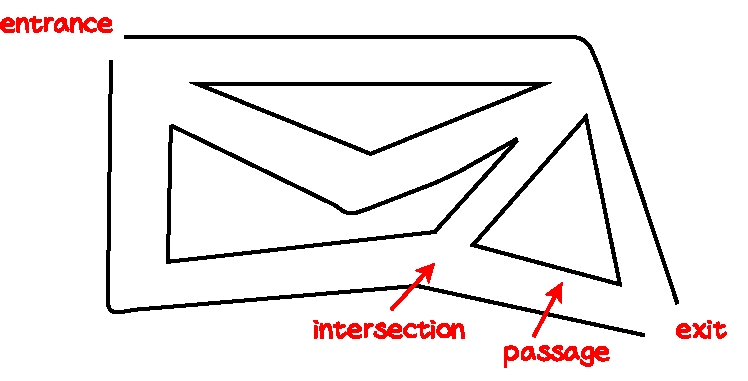
\includegraphics[width=7cm, height=4cm]{week12/maze.pdf}
		\column{0.5\textwidth}

		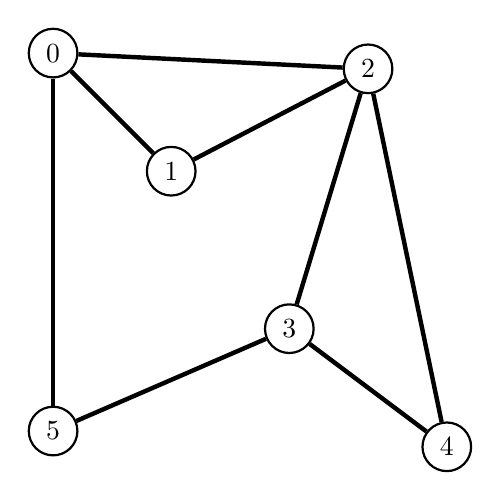
\begin{tikzpicture}
			\begin{scope}[every node/.style={circle,thick,draw}]
				\node (A) at (0,3) {0};
				\node (B) at (1.5,1.5) {1};
				\node (C) at (4,2.8) {2};
				\node (D) at (3,-.5) {3};
				\node (E) at (5,-2) {4};
				\node (F) at (0,-1.8) {5} ;
			\end{scope}

			\begin{scope}[>={Stealth[black]},
				every node/.style={fill=white,circle},
				every edge/.style={draw, ultra thick}]
				\path  (A) edge  (B);
				\path  (A) edge  (C);
				\path  (E) edge  (D);
				\path  (A) edge  (F);
				\path  (F) edge  (D);
				\path (C) edge (B);
				\path (C) edge (D);
				\path (C) edge (E);
			\end{scope}
		\end{tikzpicture}

	\end{columns}
\end{frame}

\begin{frame}[fragile]
	\frametitle{Depth-first search (DFS)}

	\begin{block}{DFS}
		Depth-first search (DFS) is an algorithm for traversing or searching tree or graph data structures. The algorithm starts at the root node (selecting some arbitrary node as the root node in the case of a graph) and explores \alert{as far as possible} along each branch before \alert{backtracking}.
	\end{block}
\end{frame}


\begin{frame}[fragile]
	\frametitle{Revisit tree traversal}

	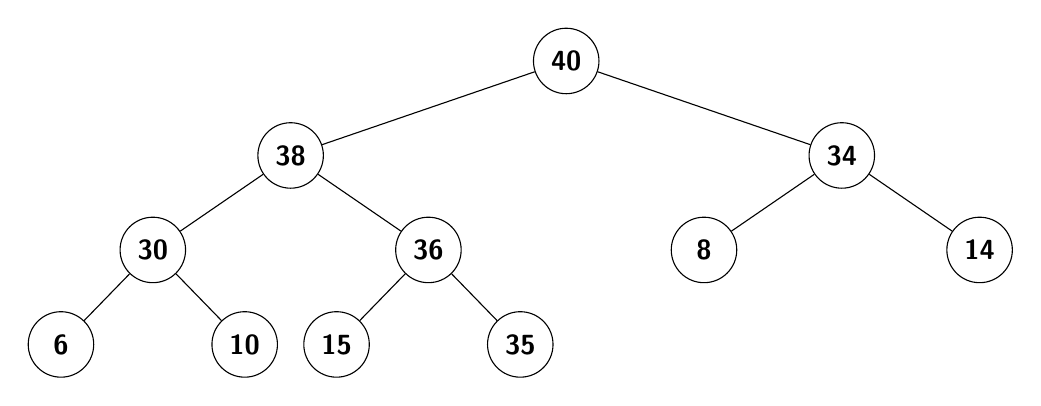
\begin{tikzpicture}[  treenode/.style = {align=center, inner sep=1pt, text centered,
					font=\sffamily},
			bst/.style = {treenode, circle, black, font=\sffamily\bfseries, draw=black, text width=2em},
			txt/.style = {text width=1.5em, red},
			rugularline/.style={edge from parent/.style={black, line width=0.2mm, draw}},
			noline/.style={edge from parent/.style={black, line width=0.2mm}},
			level/.style={sibling distance = 7cm/#1,
					level distance = 1.2cm}
		]
		\node [bst] (3n1) {40}
		child {node [bst] {38}
				child {node [bst] {30}
						child {node [bst] {6}}
						child {node [bst] {10}}
					}
				child  {node [bst] {36}
						child  {node [bst] {15}}
						child {node  [bst] {35}}
					}
			}
		child { node [bst] {34}
				child{node [bst] {8}}
				child{node [bst] {14}}
			}
		;
	\end{tikzpicture}

	Compare pre-order traversal and \alert{DFS}. See more at \href{https://en.wikipedia.org/wiki/File:Depth-First-Search.gif}{Wikipedia}.
\end{frame}


\begin{frame}[fragile]
	\section{\textcolor{darkmidnightblue}{Search}}

	\begin{minted}[bgcolor=LightGray, fontsize=\small]{python}
class Search:
  def __init__(self, G, s):
      pass
  def marked(self, v):
     """is v connected to s?""" 
  def count(self):
     """how many vertices are connected to s?""" 
  \end{minted}

\end{frame}

\begin{frame}[fragile]
	\frametitle{2.1 DFS}
	\begin{columns}
		\column{0.5\textwidth}
		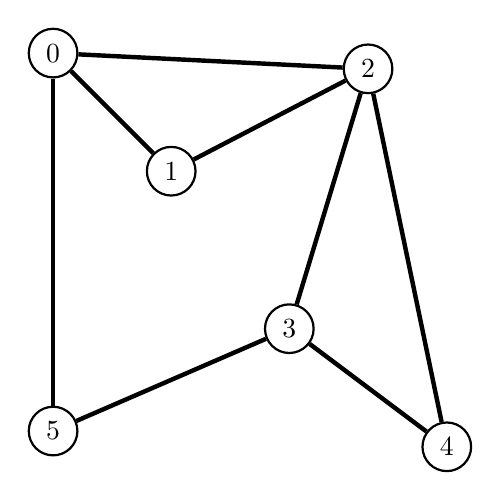
\begin{tikzpicture}
			\begin{scope}[every node/.style={circle,thick,draw}]
				\node (A) at (0,3) {0};
				\node (B) at (1.5,1.5) {1};
				\node (C) at (4,2.8) {2};
				\node (D) at (3,-.5) {3};
				\node (E) at (5,-2) {4};
				\node (F) at (0,-1.8) {5} ;
			\end{scope}

			\begin{scope}[>={Stealth[black]},
				every node/.style={fill=white,circle},
				every edge/.style={draw, ultra thick}]
				\path  (A) edge  (B);
				\path  (A) edge  (C);
				\path  (E) edge  (D);
				\path  (A) edge  (F);
				\path  (F) edge  (D);
				\path (C) edge (B);
				\path (C) edge (D);
				\path (C) edge (E);
			\end{scope}
		\end{tikzpicture}

		\column{0.5\textwidth}
		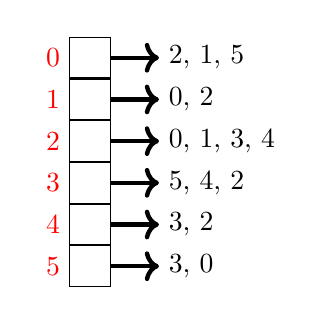
\begin{tikzpicture}
			\matrix[
				vertex/.style = {font=\sffamily\bfseries, draw=black, text width=.8em, text height=.8em, align=center},
				txt/.style = {text width=.5em, red},
			]
			{
				\node[txt]{0}; & \node[vertex](v0){};  \\
				\node[txt]{1}; & \node[vertex](v1) {}; \\
				\node[txt]{2}; & \node[vertex](v2) {}; \\
				\node[txt]{3}; & \node[vertex](v3) {}; \\
				\node[txt]{4}; & \node[vertex](v4) {}; \\
				\node[txt]{5}; & \node[vertex](v5) {}; \\
			};


			\begin{scope}[every node/.style={xshift=2em, text width=4em},]
				\node[right of=v0,] (adj0) {2, 1, 5};
				\draw[->, ultra thick] (v0) -- (adj0);
				\node[right of=v1,] (adj1) {0, 2};
				\draw[->, ultra thick] (v1) -- (adj1);
				\node[right of=v2,] (adj2) {0, 1, 3, 4};
				\draw[->, ultra thick] (v2) -- (adj2);
				\node[right of=v3,] (adj3) {5, 4, 2};
				\draw[->, ultra thick] (v3) -- (adj3);
				\node[right of=v4,] (adj4) {3, 2};
				\draw[->, ultra thick] (v4) -- (adj4);
				\node[right of=v5,] (adj5) {3, 0};
				\draw[->, ultra thick] (v5) -- (adj5);
			\end{scope}


		\end{tikzpicture}
	\end{columns}
\end{frame}

\begin{frame}[fragile]
	\begin{enumerate}
		\item To visit a vertex, mark it as visited.
		\item Visit (recursively) all the unvisited vertices adjacent to it.
	\end{enumerate}
	\begin{minted}[bgcolor=LightGray, fontsize=\small]{python}
class Search:
    def __init__(self, g: Graph, s):
        self._marked = [False] * g.v()
        self._count = 0
        self.dfs(g, s)

    def dfs(self, g: Graph, v):
        self._marked[v] = True
        self._count += 1
        for w in g.adj(v):
            if not self._marked[w]:
                self.dfs(g, w)
  \end{minted}
\end{frame}

\begin{frame}[fragile]
	\frametitle{Check connectivity}
	\begin{enumerate}
		\item How to design an algorithm to check whether two vertices are connected?
		\item If two vertices are connected, how to find the path between them?
	\end{enumerate}
\end{frame}

\begin{frame}[fragile]
	\frametitle{2.2 Finding paths}

	\begin{minted}[bgcolor=LightGray, fontsize=\small]{python}
class Paths:
    def __init__(self, g, s):
      pass

    def has_path_to(self, v):
      """is there a path from s to v?"""

    def path_to(self, v):
      """path from s to v; None if no such path"""
  \end{minted}
\end{frame}

\begin{frame}[fragile]
	\begin{columns}
		\column{0.5\textwidth}
		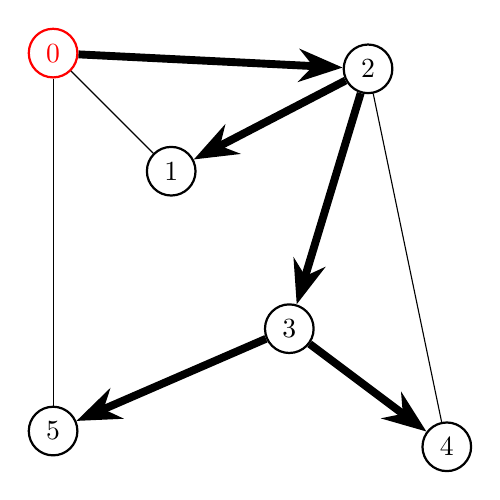
\begin{tikzpicture}
			\begin{scope}[every node/.style={circle,thick,draw}]
				\node[red] (A) at (0,3) {0};
				\node (B) at (1.5,1.5) {1};
				\node (C) at (4,2.8) {2};
				\node (D) at (3,-.5) {3};
				\node (E) at (5,-2) {4};
				\node (F) at (0,-1.8) {5} ;
			\end{scope}

			\begin{scope}[>={Stealth[black]},
				every node/.style={fill=white,circle},
				every edge/.style={draw}]
				\path  (A) edge  (B);
				\path[->, line width=1mm] (A) edge  (C);
				\path [->, line width=1mm]  (D) edge  (E);
				\path  (A) edge  (F);
				\path [->, line width=1mm]  (D) edge  (F);
				\path [->, line width=1mm] (C) edge (B);
				\path [->, line width=1mm] (C) edge (D);
				\path (C) edge (E);
			\end{scope}
		\end{tikzpicture}
		\column{0.5\textwidth}
		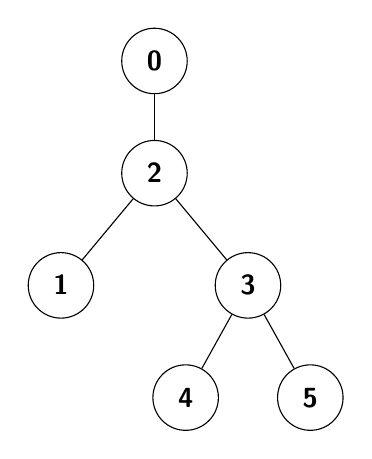
\begin{tikzpicture}[treenode/.style = {align=center, inner sep=1pt, text centered, font=\sffamily}, bst/.style = {treenode, circle, black, font=\sffamily\bfseries, draw=black, text width=2em},level/.style={sibling distance = 5cm/#1,
						level distance = 1.5cm}, scale=.95, ]
			\node [bst] {0}
			child {node [bst] {2}
					child {node [bst] {1}
						}
					child {node [bst] {3}
							child {node [bst] {4}}
							child {node [bst] {5}}
						}
				}
			;
		\end{tikzpicture}
	\end{columns}
	To track the path, we can use \alert{edgeTo} array in which \texttt{edgeTo[v]} means the last vertex on known path to $v$.
\end{frame}

\begin{frame}[fragile]
	\frametitle{dfs}

	\begin{minted}[bgcolor=LightGray, fontsize=\small]{python}
    def dfs(self, graph: Graph, v):
        self._marked[v] = True
        for w in graph.adj(v):
            if not self._marked[w]:
                self._edge_to[w] = v
                self.dfs(graph, w)
  \end{minted}

	How to find the path from $s$ to $v$ based on \texttt{edgeTo} array?
\end{frame}

\begin{frame}[fragile]
	\begin{minted}[bgcolor=LightGray, fontsize=\small]{python}
    def path_to(self, v):
        if not self.has_path_to(v):
            return None
        path = []
        x = v
        while x != self._source:
            path.append(x)
            x = self._edge_to[x]
        path.append(self._source)
        return path
  \end{minted}
\end{frame}

\begin{frame}[fragile]
	\frametitle{Exercise}
	Given an undirected graph with $E$ edges and $V$ vertices, we run a DFS algorithm on it. Which of the following statements are true?

	\begin{enumerate}
		\item The algorithm runs in $O(|E| + |V|)$ time.
		\item The paths discovered by the algorithm are the shortest paths.
		\item The paths discovered by the algorithm are the longest paths.
		\item The paths discoverer by the algorithm depend on the representations of the graph.
	\end{enumerate}
\end{frame}

\begin{frame}[fragile]
	\frametitle{2.3 Breadth-first search (BFS)}
	\begin{block}{BFS}
		It starts at the tree root and explores all nodes at the present depth prior to moving on to the nodes at the next depth level.
	\end{block}

	\begin{center}
		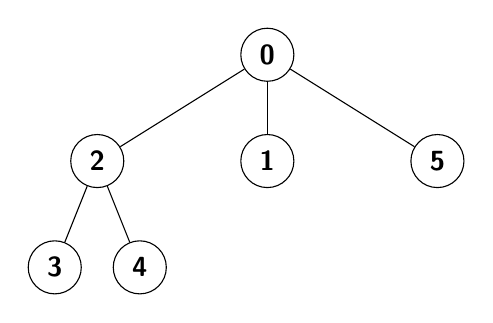
\begin{tikzpicture}[treenode/.style = {align=center, inner sep=1pt, text centered, font=\sffamily}, bst/.style = {treenode, circle, black, font=\sffamily\bfseries, draw=black, text width=1.5em},level/.style={sibling distance = 2.4cm/#1,
						level distance = 1.5cm}, scale=.9, ]
			\node [bst] {0}
			child {node [bst] {2}
					child {node [bst] {3}
						}
					child {node [bst] {4}
						}
				}
			child {node [bst] {1}}
			child {node [bst] {5}}
			;
		\end{tikzpicture}
		As for a tree, it is also known as \alert{level-order} traversal.
	\end{center}
\end{frame}

\begin{frame}[fragile]

	\begin{columns}
		\column{0.5\textwidth}
		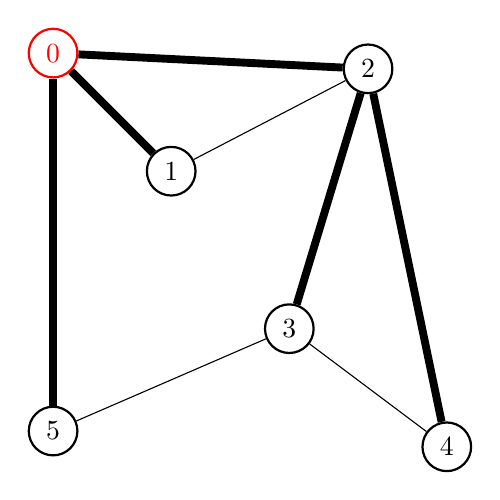
\begin{tikzpicture}
			\begin{scope}[every node/.style={circle,thick,draw}]
				\node[red] (A) at (0,3) {0};
				\node (B) at (1.5,1.5) {1};
				\node (C) at (4,2.8) {2};
				\node (D) at (3,-.5) {3};
				\node (E) at (5,-2) {4};
				\node (F) at (0,-1.8) {5} ;
			\end{scope}

			\begin{scope}[>={Stealth[black]},
				every node/.style={fill=white,circle},
				every edge/.style={draw}]
				\path[line width=1mm]  (A) edge  (B);
				\path[line width=1mm] (A) edge  (C);
				\path (D) edge  (E);
				\path [line width=1mm] (A) edge  (F);
				\path   (D) edge  (F);
				\path (C) edge (B);
				\path [line width=1mm] (C) edge (D);
				\path [line width=1mm](C) edge (E);
			\end{scope}
		\end{tikzpicture}
		\column{0.5\textwidth}
		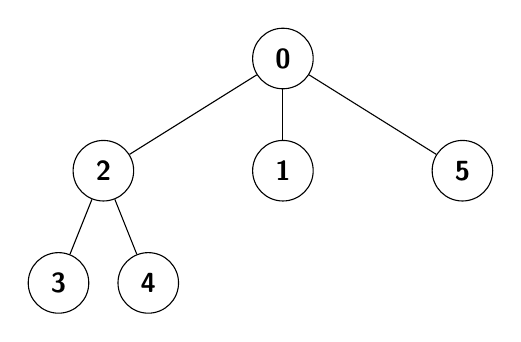
\begin{tikzpicture}[treenode/.style = {align=center, inner sep=1pt, text centered, font=\sffamily}, bst/.style = {treenode, circle, black, font=\sffamily\bfseries, draw=black, text width=1.8em},level/.style={sibling distance = 2.4cm/#1,
						level distance = 1.5cm}, scale=.95, ]
			\node [bst] {0}
			child {node [bst] {2}
					child {node [bst] {3}
						}
					child {node [bst] {4}
						}
				}
			child {node [bst] {1}}
			child {node [bst] {5}}
			;
		\end{tikzpicture}
	\end{columns}
\end{frame}

\begin{frame}[fragile]
	\begin{minted}[bgcolor=LightGray, fontsize=\small]{python}
def bfs(self, graph: Graph, s):
    q = queue()
    q.enqueue(s)
    self._marked[s] = True
    while queue:
        v = q.dequeue()
        for w in graph.adj(v):
            if not self._marked[w]:
                self._marked[w] = True
                self._edge_to[w] = v
                q.enqueue(w)
  \end{minted}
	How about the time complexity of BFS?
\end{frame}

\begin{frame}
	\begin{block}{Proposition}
		For any vertex $v$ reachable from $s$, the BFS algorithm computes a path from $s$ to $v$ with the fewest number of edges (\alert{the shortest path}).
	\end{block}
\end{frame}

\begin{frame}[fragile]
	\frametitle{Exercise}
	Consider a maze with a starting point and an endpoint represented by a 2D array containing 0s and 1s, where 0 denotes a pathway and 1 denotes a wall. Design an algorithm using Breadth-First Search (BFS) to determine whether there exists a path from the starting point to the endpoint.


\end{frame}

\begin{frame}[fragile]

	\begin{minted}[bgcolor=LightGray, fontsize=\small]{python}
[
  [0, 1, 0, 0, 0],
  [0, 1, 0, 1, 0],
  [0, 0, 0, 1, 0],
  [1, 1, 1, 1, 0],
  [0, 0, 0, 0, 0]
]
  \end{minted}

	The starting point is at the top-left corner (0, 0), and the endpoint is at the bottom-right corner (4, 4).
\end{frame}

\begin{frame}[fragile]
	\frametitle{Application: Connected components}
	\begin{block}{Definition}
		A graph is \alert{connected} if there is a path from every vertex to every other in the graph. A graph that is \emph{not connected} consists of a set of \alert{connected components}, which are maximal connected subgraphs.
	\end{block}

	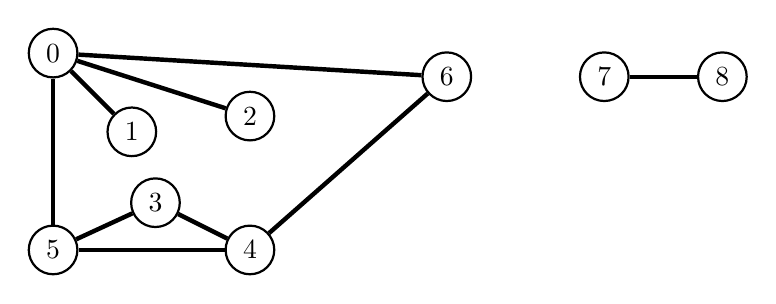
\begin{tikzpicture}
		\begin{scope}[every node/.style={circle,thick,draw}]
			\node (A) at (0,3.3) {0};
			\node (B) at (1,2.3) {1};
			\node (C) at (2.5,2.5) {2};
			\node (D) at (1.3,1.4) {3};
			\node (E) at (2.5,.8) {4};
			\node (F) at (0, .8) {5} ;
			\node (G) at (5, 3) {6} ;
			\node (H) at (7, 3) {7};
			\node (I) at (8.5, 3) {8};
		\end{scope}

		\begin{scope}[>={Stealth[black]},
			every node/.style={fill=white,circle},
			every edge/.style={draw, ultra thick}]
			\path  (A) edge  (B);
			\path  (A) edge  (C);
			\path  (E) edge  (D);
			\path  (A) edge  (F);
			\path  (F) edge  (E);
			\path  (F) edge  (D);
			\path  (A) edge  (G);
			\path  (G) edge  (E);
			\path (H) edge (I);
		\end{scope}
	\end{tikzpicture}
\end{frame}


\begin{frame}

	\section{\textcolor{darkmidnightblue}{Conclusion}}
	\begin{enumerate}
		\item Graph
		\item DFS
		\item BFS
	\end{enumerate}
\end{frame}
\end{document}
